\documentclass[12pt]{article}

\usepackage[sorting=none]{biblatex}
\usepackage{indentfirst}
\usepackage{graphicx}
\usepackage{mwe}
\usepackage{wrapfig}
\addbibresource{bib.bib}

\begin{document}
\begin{center}
{\large \textbf{\textsc{CS-445/545 Machine Learning Final: CNN versus SVM}}}

\bigskip

\textsc{Will Farris, Ajay Babu Gorantla, Gilbert Grundy, Kuldeep Akbari, Joel Williams}
\end{center}

\section{Abstract}

Machine learning is a notoriously data-hungry field within computer science. Often, the effectiveness of a machine learning program hinges on the volume of data fed into it. Choosing a model which performs well under data constraints, then, can boost a model’s performance when data is scarce. Convolutional neural networks (CNNs) are used by many modern image processing applications to classify images. Support vector machines (SVNs) can also be used, however CNNs tend to be used more commonly. Our research pits CNNs and SVNs against one another, to see which one performs classification better on a subset of the MNIST fashion dataset using various performance metrics. We first optimize a CNN and an SVM by tweaking various hyperparameters, and then compare their relative performance as training data size scales.

\section{Introduction}

Machine learning algorithms for image classification have been steadily gaining wide advances since their inception, due to ever increasing compute power and the continuously accumulating amount of data on the internet. Researchers in the 1960s conceived of using Markov chains to perform contextual classification of an image using binary array values \cite{1053827}. In 1968, researchers also explored using discrete probability trees for image classification, producing a maximum-likelihood estimation \cite{chow1968approximating}. In 1995, Vladmir Vapnik at Bell Labs invented support vector machines with binary classification \cite{cortes1995support}. The usual approach for multiclass classification for SVMs is to break the classification into multiple binary sub-problems. CNNs are evolutionary descendents of perceptrons and multilayer neural networks. The first generation of CNNs were based off of the “neocognitron”, created by Kunihito Fukushima, who published the results in \textit{Biological Cybernetics} \cite{fukushima1982neocognitron}. This helped spur the Deep Learning revolution, especially in regards to the widespread use of machine learning algorithms for internet image classification.

Our research pits these two learning algorithms against each other. Our intention is to first optimize each algorithm individually, by varying hyperparameters on each to maximize their accuracy performance. Then we contrasted the optimized models, the CNN and the SVM, to see which performs better with different sized training sets. With CNN, we’ll vary the number of hidden layers, the learning rate, and activation function. We kept our momentum rate constant at 0.2 . With the SVM, we varied using different kernels between linear, sigmoid, 3rd order polynomial, and radial basis function (RBF). Since both algorithms are extremely architecturally different, for instance the SVM has no concept of learning rate or momentum, direct comparisons between the two by varying hyperparameters isn’t the most productive experimentation method. Instead, we compare accuracy between our optimized hyperparameter models, contrasting their performance on controlled size training sets. We hope that this will provide future machine learning practitioner intuitions regarding which algorithm to use given a particularly sized training set.

\section{CNN Analysis}

For the analysing of the CNN we are varying the number of hidden layers, activation functions, and the learning rates. The CNN uses 10 epochs of training data and a batch size of 100. 

\subsection{Depth}

First, we compared the accuracy of the CNN with a varied amount of hidden layers with 32 ReLu nodes each. We set the learning rate (0.1) and activation function (ReLU)

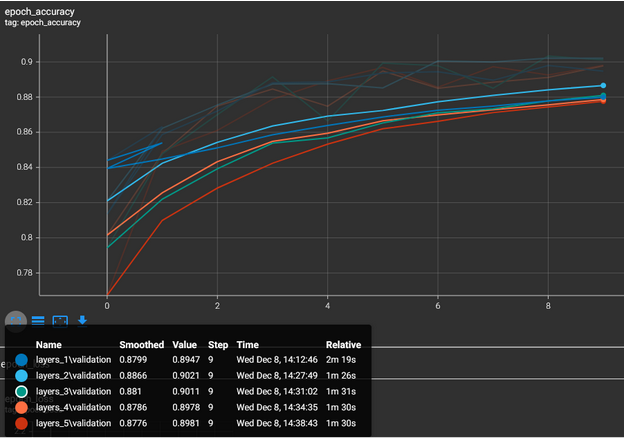
\includegraphics[scale=.75]{cnngraph1.PNG}

As we can observe, there is not much difference in the final accuracies for change in the number of hidden(Dense) layers.

Among the different models(each with a different number of hidden layers),after 10 epochs, the model with 2 hidden(Dense) layers had the best accuracy on the validation set i.e. 90.21% .

We wanted to analyze how that above best(in terms of accuracy) model would behave with a change in the learning rate. In the next section, we talk about that behavior.

\subsection{Learning}
We then compared training rates of 0.1, 0.01, 0.001, and 0.0001.

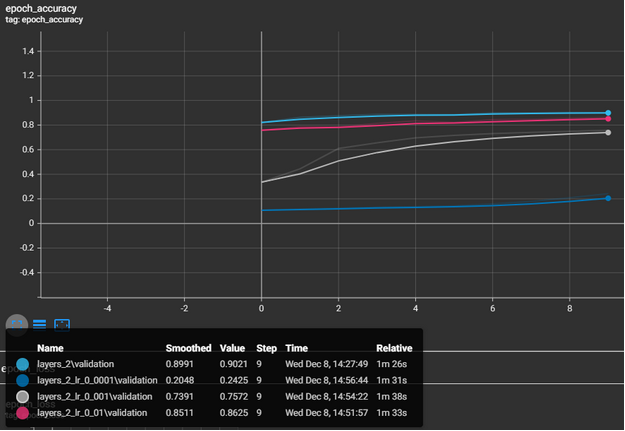
\includegraphics[scale=.75]{cnngraph2.PNG}

We can clearly observe that, with increase in the learning rate the accuracy is also increasing. The lowest accuracy was obtained with learning rate =0.0001 and the highest accuracy was obtained with learning rate = 0.1

So, among the different tested models with change in network size(depth) and change in learning rate, the best model we found out was the model that has 2 hidden(Dense) layers and with learning rate 0.1

Now, we wanted to analyze the behavior of the above model with change in type of activation function. In the next section, we talk about that behavior.

\subsection{Activation Functions}

Finally, we compared the activation functions of ReLU, Sigmoid and tanh.

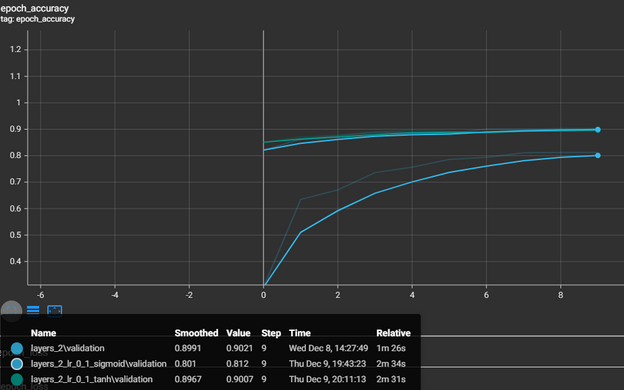
\includegraphics[scale=.75]{cnngraph3.PNG}

From the above plot, we inferred that all the activation functions gave some good results. However, ‘ReLU’ and ‘tanh’ played out relatively and considerably better than the ‘Sigmoid’. There is a very slight difference between the accuracies of ‘ReLU’ and ‘tanh’. 

\bigskip

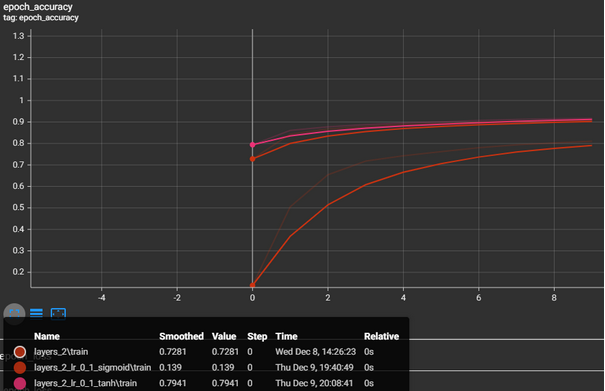
\includegraphics[scale=.77]{cnngraph4.PNG}

\newpage

One interesting observation that we noticed from the above figure is that ‘tanh’ started off with better training accuracies than the other two activation functions. Although there is a very slight difference in accuracy between ‘tanh’ and ‘ReLU', the latter has better accuracy, the main reason we chose to consider ‘ReLU’ for further analysis is that it is computationally less expensive than ‘tanh’.

\section{SVM Analysis}

We implemented a support vector machine using scikit-learn which we then trained on the fashion mnist dataset. We tested the accuracy of three different kernel functions with varying amounts of training data for a support vector machine implemented with scikit-learn. Of the four kernel functions tested, the radial basis function resulted in the highest test accuracy at 88.36\% when provided 60,000 training samples. The sigmoid function came dead last, settling at 70.74\%, it was the only kernel function that descended in accuracy as the training samples increased. The linear kernel function performed the next worst at 83.7\% test accuracy, and the 3rd degree polynomial kernel came in a close second at 87.55\%.

\subsection{Kernels used}

To choose the most performant SVM we compared the relative performance of the following several kernel functions. As different kernel functions are suited for different distributions of data, we wanted to choose a kernel which would be most performant on the task of image recognition. We compared the performance of the following kernel function: radial basis function (RBF), 3rd degree polynomial, linear and sigmoid. Experimenting with the kernel function used allowed us to choose the best SVM configuration for the task of image classification.

\subsection{Results}

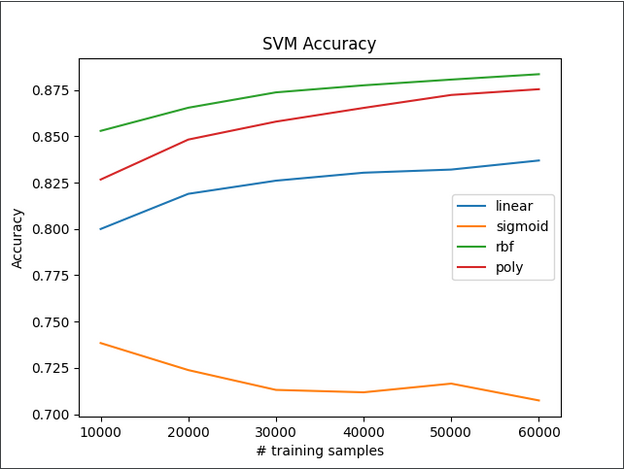
\includegraphics[scale=.75]{svmgraph1.PNG} 






\end{document}
